
% \section{...} 
%   \usepackage[utf8]{inputenc}
%   \usepackage[T1]{fontenc}
%   \usepackage[spanish]{babel}
%   \usepackage{amsmath}
%   \usepackage{booktabs}
%   \usepackage{multirow}
%   \usepackage{graphicx}
% Las figuras deben estar en la misma carpeta que el .tex:
%   fig_temperatura.png, fig_humedad.png, fig_velocidad.png
% ============================================================
\documentclass[11pt]{article}
\usepackage[utf8]{inputenc}
\usepackage[T1]{fontenc}
\usepackage[spanish]{babel}
\usepackage{amsmath}
\usepackage{booktabs}
\usepackage{multirow}
\usepackage{graphicx}
\usepackage[margin=2.5cm]{geometry}

\begin{document}

\section{Definición de variables, fuzzificación y conjuntos difusos}

\subsection{Variables del sistema}

El sistema de control difuso del ventilador cuenta con dos variables de entrada y una de salida. La Tabla~\ref{tab:variables} resume sus universos del discurso, unidades y conjuntos difusos.

\begin{table}[h]
\centering
\caption{Variables de entrada y salida del sistema.}
\label{tab:variables}
\begin{tabular}{llcp{2.6cm}l}
\toprule
\textbf{Variable} & \textbf{Tipo} & \textbf{Universo} & \textbf{Unidad} & \textbf{Conjuntos difusos} \\
\midrule
Temperatura & Entrada & $[10, 40]$ & $^\circ$C & Fría, Templada, Caliente \\
Humedad relativa & Entrada & $[0, 100]$ & \% & Baja, Media, Alta \\
Velocidad del ventilador & Salida & $[0, 100]$ & \% de la velocidad máxima & Baja, Media, Alta \\
\bottomrule
\end{tabular}
\end{table}

\subsection{Funciones de pertenencia}

Se utilizaron funciones trapezoidales y triangulares. La función trapezoidal con parámetros $(a, b, c, d)$ se define como:
\[
\mu(x) =
\begin{cases}
0, & x \le a \ \text{ o } \ x \ge d, \\[4pt]
\dfrac{x - a}{b - a}, & a < x < b, \\[8pt]
1, & b \le x \le c, \\[4pt]
\dfrac{d - x}{d - c}, & c < x < d.
\end{cases}
\]

La función triangular $(a, b, c)$ es el caso particular en que $b = c$. En los conjuntos de los extremos se cumple $a = b$ o $c = d$, por lo que tienen una sola pendiente. Los parámetros de cada conjunto se muestran en la Tabla~\ref{tab:parametros}.

\begin{table}[h]
\centering
\caption{Parámetros de las funciones de pertenencia.}
\label{tab:parametros}
\begin{tabular}{llcc}
\toprule
\textbf{Variable} & \textbf{Conjunto} & \textbf{Tipo} & \textbf{Parámetros} \\
\midrule
\multirow{3}{*}{Temperatura ($^\circ$C)} & Fría & Trapecio & $(10, 10, 16, 22)$ \\
 & Templada & Triángulo & $(18, 24, 30)$ \\
 & Caliente & Trapecio & $(26, 32, 40, 40)$ \\
\midrule
\multirow{3}{*}{Humedad (\%)} & Baja & Trapecio & $(0, 0, 25, 50)$ \\
 & Media & Triángulo & $(30, 50, 70)$ \\
 & Alta & Trapecio & $(50, 75, 100, 100)$ \\
\midrule
\multirow{3}{*}{Velocidad (\%)} & Baja & Trapecio & $(0, 0, 20, 45)$ \\
 & Media & Triángulo & $(30, 50, 70)$ \\
 & Alta & Trapecio & $(55, 80, 100, 100)$ \\
\bottomrule
\end{tabular}
\end{table}

Las Figuras 1, 2 y 3 muestran las funciones de pertenencia de cada variable. En las dos primeras se marcan los valores de ejemplo usados en la siguiente subsección.

\begin{center}
\begin{minipage}{\textwidth}
\centering
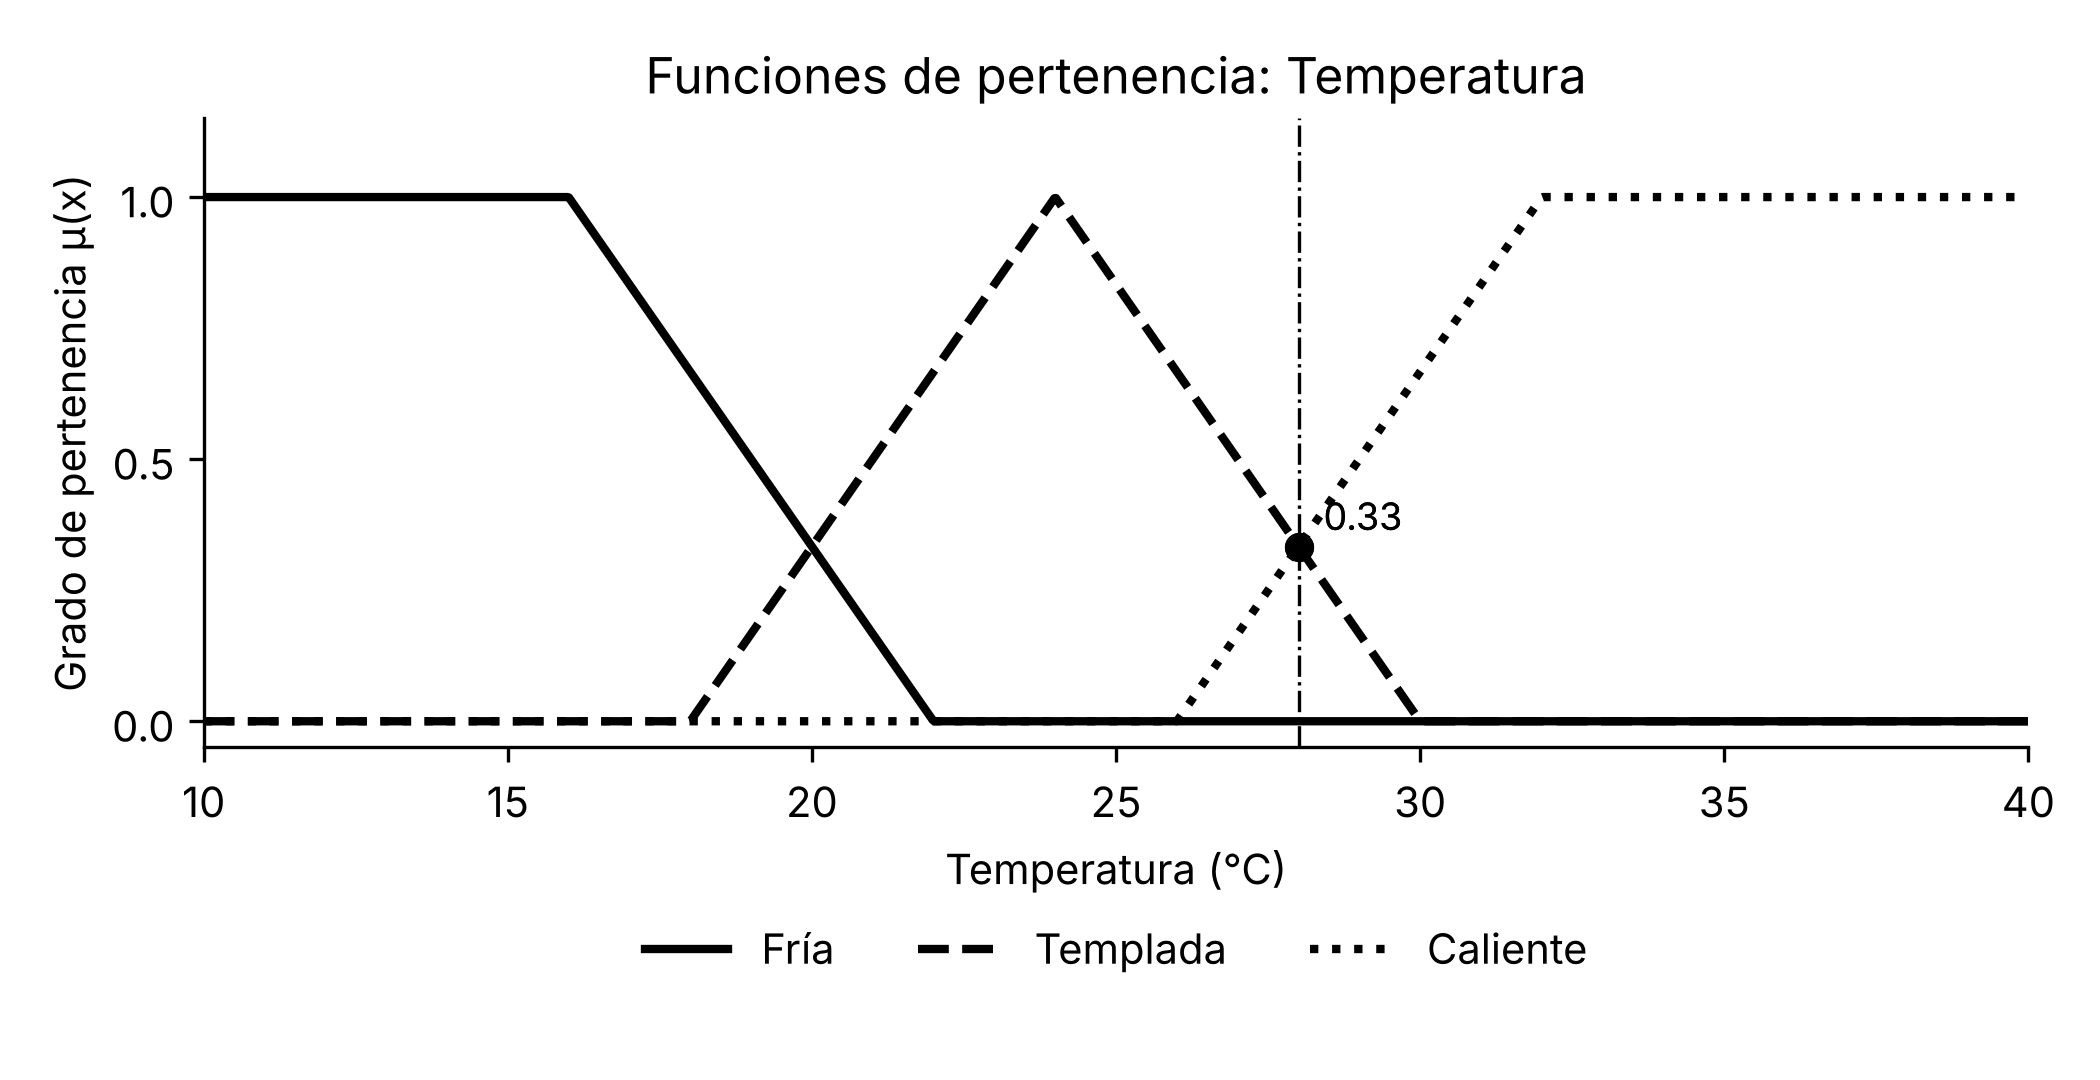
\includegraphics[width=0.7\textwidth]{fig_temperatura.png}\par
\small Figura 1. Funciones de pertenencia de la temperatura.
\end{minipage}

\vspace{1em}

\begin{minipage}{\textwidth}
\centering
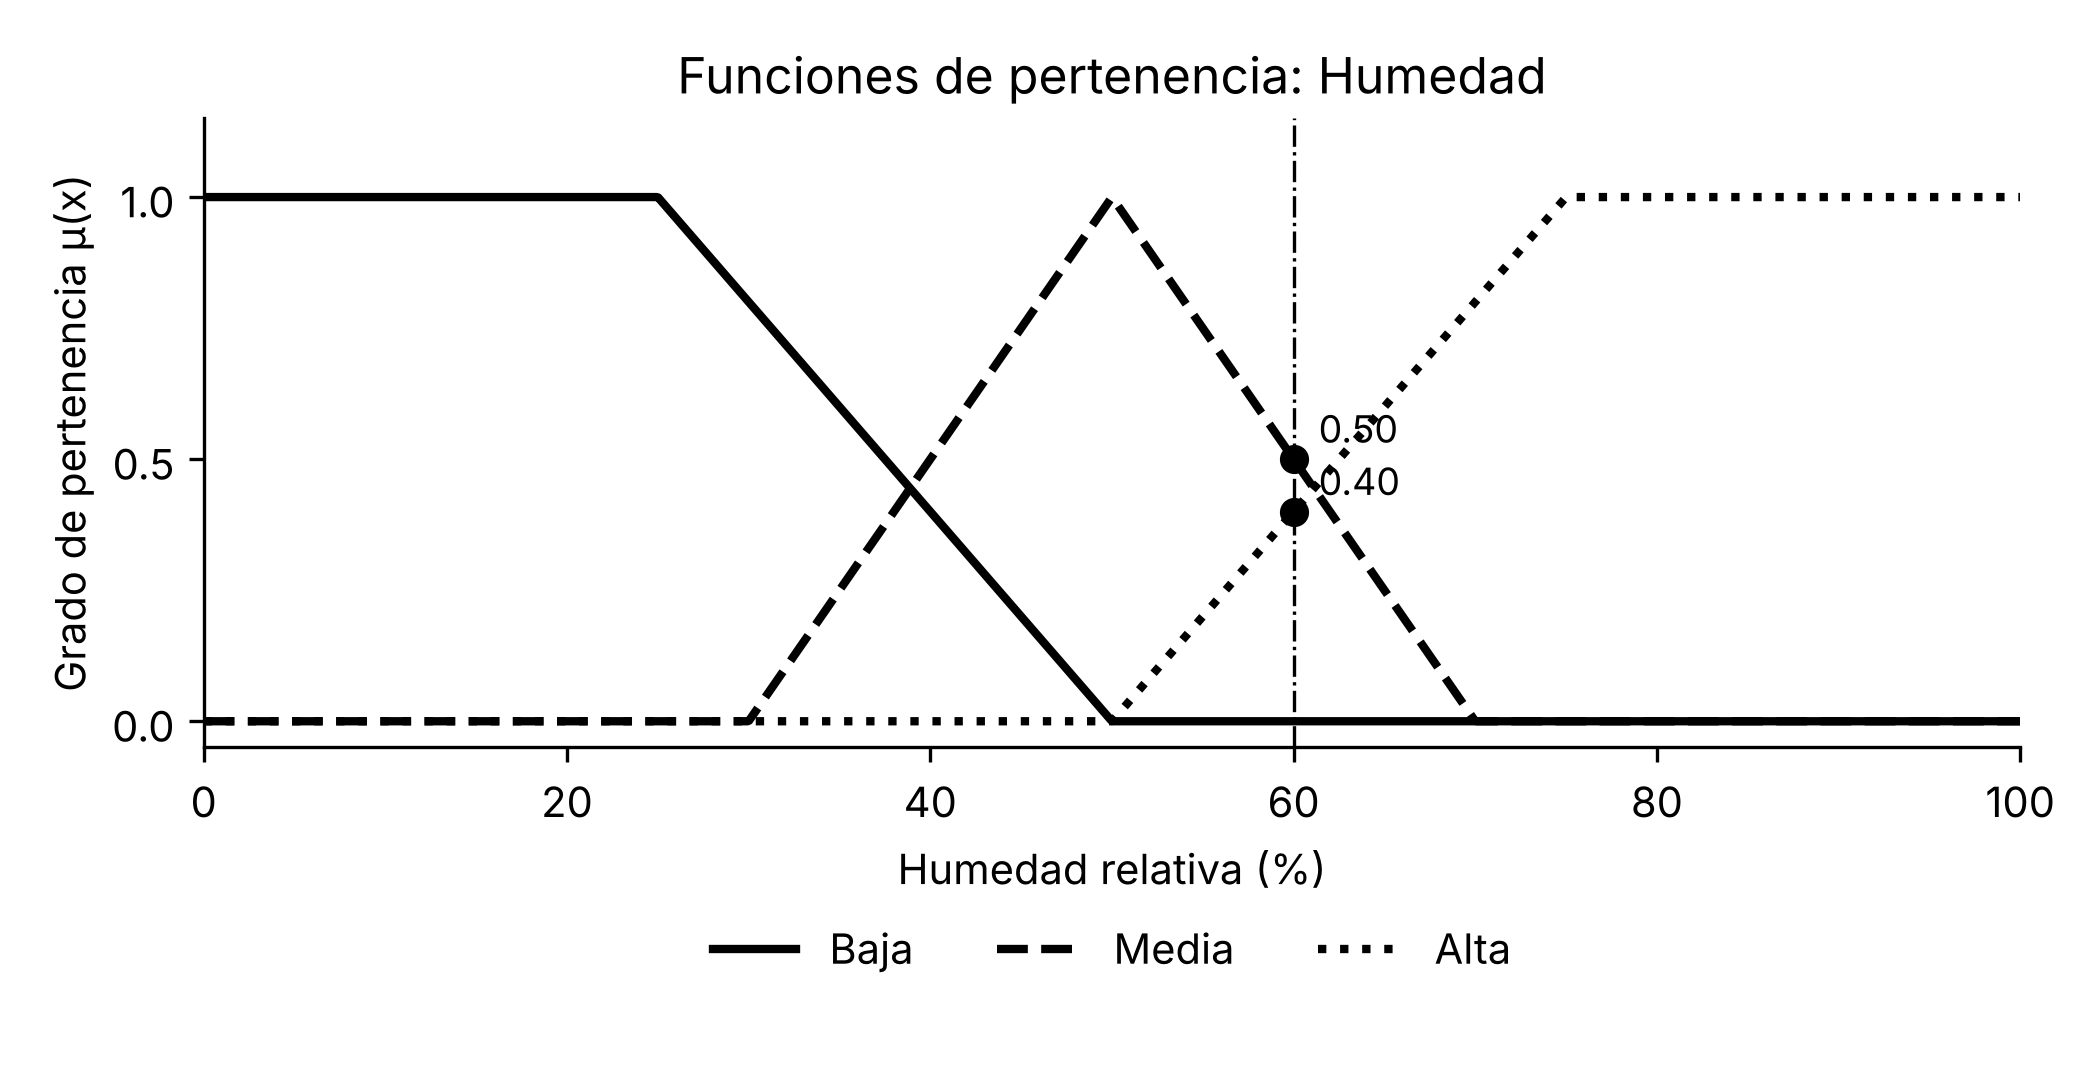
\includegraphics[width=0.7\textwidth]{fig_humedad.png}\par
\small Figura 2. Funciones de pertenencia de la humedad relativa.
\end{minipage}

\vspace{1em}

\begin{minipage}{\textwidth}
\centering
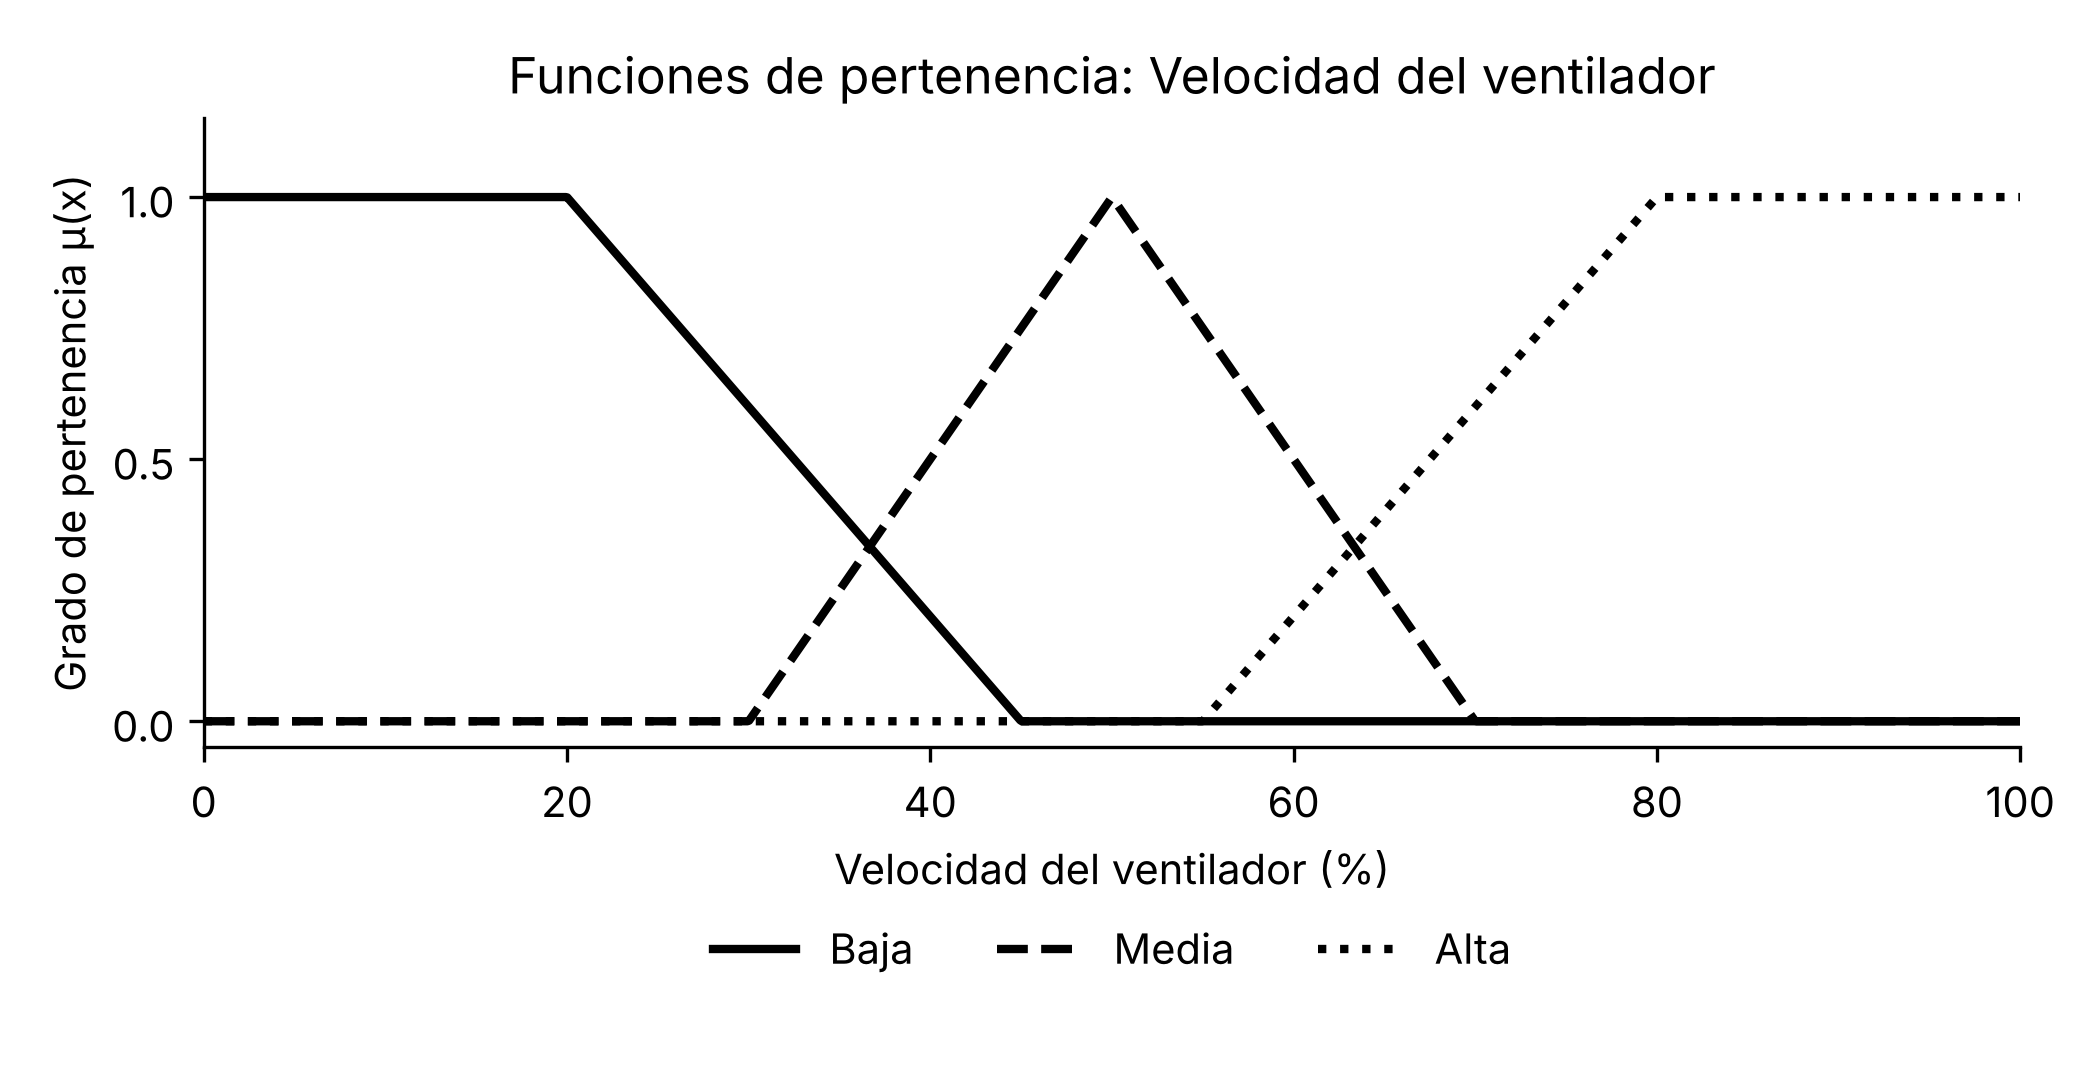
\includegraphics[width=0.7\textwidth]{fig_velocidad.png}\par
\small Figura 3. Funciones de pertenencia de la velocidad del ventilador (variable de salida).
\end{minipage}
\end{center}

\subsection{Fuzzificación}

La fuzzificación es el primer paso del algoritmo de control difuso. Consiste en tomar cada variable de entrada \emph{crisp}, medida por los sensores, y evaluarla en las funciones de pertenencia de sus conjuntos lingüísticos para obtener grados de pertenencia en el intervalo $[0, 1]$. A diferencia de un sistema clásico, donde un valor pertenece o no pertenece a un conjunto, aquí un mismo valor puede pertenecer parcialmente a varios conjuntos a la vez.

Por ejemplo, para una temperatura de $28\,^\circ$C y una humedad de $60\,\%$:
\begin{align*}
\mu_{\text{Fría}}(28) &= 0, &
\mu_{\text{Templada}}(28) &= \frac{30 - 28}{30 - 24} = 0.33, &
\mu_{\text{Caliente}}(28) &= \frac{28 - 26}{32 - 26} = 0.33, \\[6pt]
\mu_{\text{Baja}}(60) &= 0, &
\mu_{\text{Media}}(60) &= \frac{70 - 60}{70 - 50} = 0.50, &
\mu_{\text{Alta}}(60) &= \frac{60 - 50}{75 - 50} = 0.40.
\end{align*}

Estos grados de pertenencia son los valores que se usan como entrada en las cláusulas de Horn de la base de reglas.

\subsection{Justificación de los conjuntos elegidos}

\begin{enumerate}
  \item \textbf{Tres conjuntos por variable.} Son suficientes para describir el problema con términos que una persona usaría de forma natural (fría, templada, caliente) y mantienen la base de reglas manejable: con dos entradas de tres conjuntos cada una resultan 9 combinaciones.
  \item \textbf{Formas triangulares y trapezoidales.} Son simples de calcular y de interpretar, y su costo computacional es bajo, lo que las hace adecuadas para un controlador sencillo.
  \item \textbf{Conjuntos de los extremos con forma de trapecio.} Permiten que los valores extremos tengan pertenencia plena. Por ejemplo, cualquier temperatura menor o igual a $16\,^\circ$C es completamente fría.
  \item \textbf{Traslapes entre conjuntos vecinos.} Los conjuntos se superponen parcialmente (por ejemplo, entre $18$ y $22\,^\circ$C se es a la vez algo fría y algo templada), lo que hace que la transición entre estados sea gradual y que la velocidad del ventilador no cambie bruscamente.
  \item \textbf{Universos del discurso.} El rango de temperatura de $10$ a $40\,^\circ$C abarca las condiciones ambientales habituales en las que se usaría un ventilador. La humedad relativa se define en su rango natural de $0$ a $100\,\%$. La velocidad se expresa como porcentaje de la velocidad máxima para que el modelo no dependa de un ventilador en particular.
\end{enumerate}

\end{document}
